\chapter{Cloud Services That Could Help DevOps Toolchain}
In the chapter we introduce the implementation of our DevOps toolchain which act as the basic environment of our experiments. Then we introduce the experiment that for answering RQ1: \textbf{How could DevOps toolchain make use of current cloud services and how these services improves the DevOps toolchain.} In section 4.1 we introduce the implementation of our testing DevOps toolchain which is according to the DevOps definitions and DevOps practices we introduced at Chapter 2. In section 4.2 we discuss the cloud services selection consideration for the experiment. In section 4.3 we introduce the implementation of our experiments. Section 4.4 focuses on the experiment result.
\section{DevOps Toolchain Implementation}
Our DevOps toolchain is used to conduct experiment that could answering 2 research questions. As we mentions above, it include DevOps elements we introduced at CH2. In this section we will first introduce the composition of our DevOps toolchain, and secondly, which elements of DevOps does each components belongs to.

// Introduce our initial design of Devops toolchain

// Point out the problem, and point out the improvement can be done in the toolchain.

\section{Cloud Services that improves our DevOps toolchain}
\label{assumption}
//  Using services in AWS as example, Introduces how cloud services could improve. describe on services in one section
\subsection{Managed Container Services for Distributed Builds} 
// Describe how AWS Fargate could Help
\subsection{Serverless computing}
// Describe how AWS lambda could Help and why do we chose it
\subsection{...}
\section{Setup for the Experiments}
\subsection{Managed container services}
\subsubsection{Test task and System Description}
// This is just a draft

In this experiment we simulate the continues delivery process of a Spring Boot web application. From the experiments, we could verify our assumption in \ref{assumption}.
The continues delivery pipeline includes following steps:
\begin{enumerate}
    \item \textit{Pull from version control}: Pull the most recent change from Github repository
    \item \textit{Build}: Build the application with Gradle
    \item \textit{Test}: Automate testing with JUnit integrated in Gradle
    \item \textit{Artefact store}: Push the build artefacts to Artifactory
\end{enumerate}
\begin{figure}[h]
    \centering
    \begin{minipage}{0.45\textwidth}
        \centering
        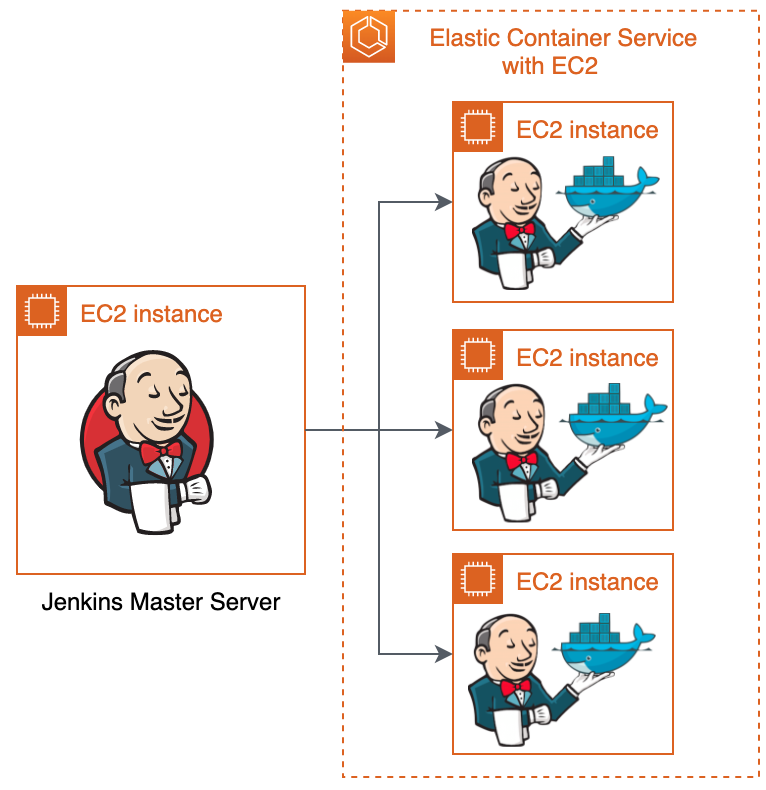
\includegraphics[width=\textwidth]{pics/jenkins-on-vm.png} % first figure itself
    \end{minipage}\hfill
    \begin{minipage}{0.54\textwidth}
        \centering
        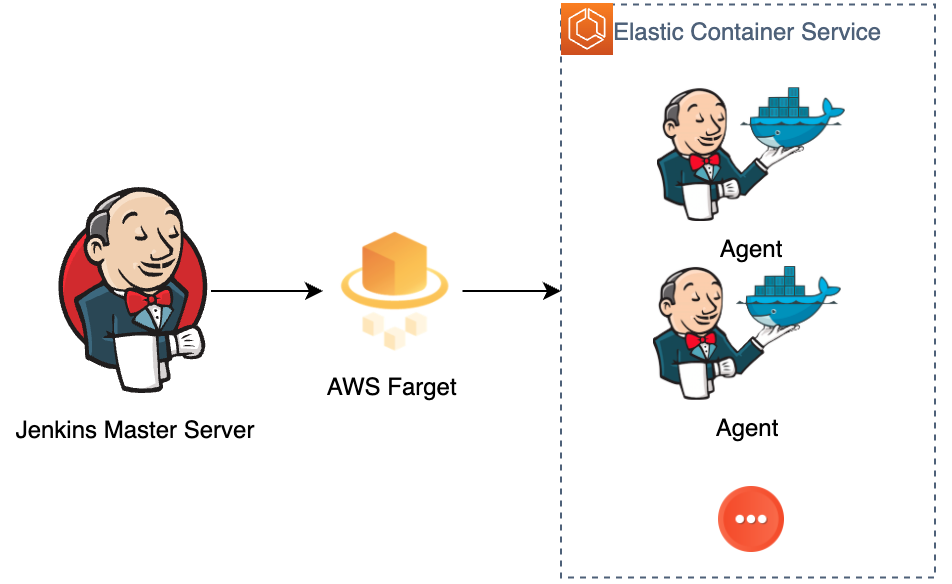
\includegraphics[width=\textwidth]{pics/jenkins-on-fargate.png} % second figure itself
    \end{minipage}
    \caption{Architecture diagram of the test Jenkins cluster with agents running in traditional virtual machine (left) and on ECS with AWS Fargate (right)}
\end{figure}
To evaluate our assumption in \ref{assumption}, we have 2 different setups. The first setup Figure 4.1 (left) is a Jenkins server with traditional virtual machine as worker agents. In the second setup Figure 4.1 (right), we use the same Jenkins server but the worker nodes is dynamically provisioned in the AWS Fargate managed cloud service.

// here write some more detail about the setup which includes IAM and hardware configuration, and also include the graph which shows the topological structure of 2 setups,

\subsubsection{Performance Properties and Evaluation}
We run the pipeline through 2 different setups, we will get the result of following properties:
\begin{itemize}
    \item \textit{Runtime} describes the total time for finishing all the tasks.
    \item \textit{Cost Structure} describes the daily cost of 2 setups under the same workload
    \item \textit{Resource Utilization} describes the average CPU/RAM usage for each instance during a single run of the pipeline.
\end{itemize}
To shows how does the 2 setups performance within the teams with different sizes, we run by run different number of tasks parallel through the pipeline. This simulates the different team size, besides, it could also shows the scalability when comes to the need of task parallelization in bigger organizations.
